\input setup_ueb

\usepackage[T1]{fontenc}


\begin{document}

\section*{Übungsaufgaben 3 \\
(Funktionen, Rekursion,Numpy, Scipy, Matplotlib )}

Hausaufgabe: Lösen Sie mindestens 6 der folgenden Aufgaben (manche Aufgaben zählen doppelt, d.h so viel wie zwei gelöste Aufgaben.)
Die Abgabe erfolgt im ISIS-Kurs, Termin wird dort bekannt gegeben.

\subsection*{Aufgaben aus dem Labor}

\begin{enumerate}[1.]
\item \textbf{Karten mischen}\\
 Bestimmen Sie durch Simulation, mit welcher Wahrscheinlichkeit beim Mischen 
eines Kartenstapels aus 52 Karten mindestens eine Karte an der alten Stelle zu liegen
kommt. Schreiben Sie dazu eine Funktion  \texttt{ziehe(l)}, die ein zufälliges Element 
der Liste l zurückgibt und dieses Element aus der Liste entfernt, eine Funktion \texttt{mische(n)},
die eine zufällige Anordnung der Zahlen $0,\ldots,n-1$ durch sukzessives Ziehen erzeugt und als Liste zurückgibt,
eine Funktion \texttt{pruefe(l)}, die True zurückgibt, falls die übergebene Anornungs-Liste eine Karte an ihrer 
alten Stelle hat (d.h. falls es ein $i$ gibt, so dass $l[i]==i$) und ein Hauptprogramm, das mit
Hilfe der Funktionen \texttt{mische} und \texttt{pruefe} das gegebene Problem löst. Für die Funktion
\texttt{ziehe} können Sie \texttt{numpy.random.randint} benutzen.\\
Zusatzfrage: Können Sie die Antwort auch auf dem Papier bestimmen?


\item \textbf{Drachenkurve}\\
Schreiben Sie ein Programm, das (mit Hilfe von Rekursion) die 
Drachenkurve zeichnet. Sie können dazu turtle-Graphik verwenden. Hinweise dazu auch auf ISIS.


\item \textbf{Kantenbild}\\
Erzeugen Sie aus einem Bild ein Schwarz-Weiß-Bild, das nur die Kanten des Bilds 
zeigt, und machen Sie das möglichst gut. Sie können dabei \texttt{scipy.ndimage}
und \texttt{scipy.misc} benutzen.


\item \textbf{Das Spiel $^*$} (zählt doppelt)\\
Schreiben Sie eine Funktion, die für das Spiel (Erklärung auf der ISIS-Seite)
mit der Ausgangsposition aus
(1,5,9) Steinen bestimmt, ob eine Position eine Siegposition ist, 
also von der aus sich durch das richtige Verhalten ein Sieg garantieren
lässt. Entsprechend schreiben Sie eine Funktion, die ermittelt,
ob eine Position eine Verlustposition ist, also ob von dort jeder 
Zug zu einer Siegposition des Gegners führt.  Außerdem ist die Position 
(0,0,0) auf jeden Fall eine Verlustposition, denn diese bedeutet,
dass der letzte Zug vom anderen Spieler gemacht wurde.
Wie erklärt, ergibt das eine rekursive Struktur.
Verwenden Sie diese Funktionen, um ein Programm zu schreiben,
dass für eine Anfangskonfiguration einen Zug empfiehlt, der zum
Sieg führt, wenn es einen solchen gibt.

Nützlich für die Programmierung wird es sein, noch eine weitere
Funktion zu schreiben, die für eine gegebene Position die Liste
der möglichen Züge, bzw. genauer der möglichen Positionen nach einem erlaubten Zug ausgibt.


\item \textbf{Fortsetzung der Wetterdatenaufgabe $^{**}$} (zählt doppelt doppelt)\\
In der Aufgabe zu den Wetterdaten vom letzten Blatt
sollten nur Eigenschaften der Temperaturdaten durch
geeignete Mittelwertbildungen (graphisch) erkennbar
werden.

Eine systematischere Art, aus den Daten Informationen
zu ziehen, ist ein \textit{Regressionsmodell}. Die vorliegenden
Daten bilden eine Messreihe. In jeder Messung $i$ der Reihe
wird (untere anderem) der Wert der Durchschnittstemperatur
\texttt{av\_temps[i]} am Tag \texttt{dates[i]} ermittelt. Wir suchen
ein Modell, dass aus dem Datum \texttt{dates[i]} die mittlere Temperatur
\texttt{av\_temps[i]} voraussagt. Das geht natürlich nicht genau,
aber wir können das Modell suchen, das den kleinsten Vorhersagefehler
macht. Bei der \glqq klassischen\grqq{} linearen Regression
werden Modelle betrachtet, bei denen die Voraussage mit Hilfe
linearer Funktionen gemacht und der Fehler durch die Summe
der Quadrate der einzelnen Fehler gemessen wird.

Für unser Beispiel wollen wir ein lineares Regressionsmodell
bauen, das einen Trend der Temperaturentwicklung unter den
jahreszeitlichen Schwankungen erkennt.

Wir bezeichen die Zielgröße \texttt{av\_temps[i]} im weiteren
als \texttt{y[i]} und in das in Tage ab einem gewissen Stichdatum umgerechnete
Datum \texttt{matplotlib.dates.date2num(dates[i])} als \texttt{x\_0[i]}.  Die (tropische)
Jahreslänge beträgt $d=365.24219052$ Tage. Wir führen Größen
$\mathtt{x\_k[i]}$ ($k=1,\ldots,366$) ein, wobei $\mathtt{x\_k[i]}$ den Wert 1 hat, wenn \texttt{dates[i]} auf den $k.$ Tag des Jahres fällt, sonst den Wert 0.
(Durch $\mathtt{np.ceil(dates\% d)}$ lässt sich das jeweilige $k$ ermitteln.)

Es sind nun Koeffizienten $\mathtt{b\_0,\ldots, b\_366}$ so zu bestimmen,
dass der quadratische Fehler
\[ \sum_i \left( \left(\sum_{k=0}^{366} \mathtt{b\_k \ x\_k[i] - y[i]}\right) \right)^2 \]
minimal wird.  $\mathrm{b\_0}$ ist als der langfristige Trend
interpretierbar, die übrigen modellieren die jahreszeitliche Schwankung.

Wenn Sie in Linearer Algebra das kleinste-Quadrate-Problem schon
behandelt haben, können Sie loslegen. Wenn nicht, ist folgende Information
nützlich: Sei $X$ die Matrix, deren Spalten die $\mathtt{x\_0,\ldots,x\_366}$ sind
und $b$ der (Spalten-) Vektor $\mathtt{(b\_0,\ldots, b\_366)}$, so ist
dasjenige $b$, das die Fehlerquadrate minimiert, durch

\[ b = (X^\top X)^{-1} X^\top y  \; \]

Verwenden Sie \texttt{numpy} und speziell \texttt{numpy.linalg}.
Welcher Trend ist aus dem Ergebnis abzulesen (Temperaturveränderung/Jahr)?

Das können Sie natürlich auch für die Maximaltemperatur und  Minimaltemperatur
machen.

Plotten sie außerdem die Koeffizienten $b[1],\ldots,b[366]$ und interpretieren
Sie den Plot.

\item \textbf{Mandelbrot-Fraktal $^*$} (zählt doppelt)\\
Die Mandelbrot-Menge ist ein vergleichsweise einfach zu generierendes Fraktal. Benannt ist es nach Bernoit Mandelbrot, der mit seiner Veröffentlichung \textit{Les objets fractals, forme, hasard et dimension} (1975) den Begriff des Fraktals geprägt hat.\\
Die Menge lebt in der Komplexen Zahlenebene und wird durch folgende Vorschrift beschrieben:
\begin{align*}
z_0 &= 0 \\
z_{n+1} &= z_n^2 + c
\end{align*}

Hier bei entspricht $c$ einem Punkt der komplexen Zahlenebene. Divergiert $z$ für $c$ nicht, gehört $c$ zur Menge. Für die Simulation lässt sich das vereinfachend durch einen fest gesetzen Maximalwert überprüfen. Numpy Arrays dürfen auch Komplexe Zahlen enthalten, wenn das Array entsprechend initialisiert wird (np.zeros((xres, yres), dtype=np.complex\textunderscore)

Empfindliche Parameter sind die Pixeldichte (startet mit 200x200) und die Interationstiefe (erst mal begrenzen auf 200). Oft wird das Fraktal in Farbverläufen dargestellt, indem man die Iterationstiefe auswertet die benötigt wird um den Maximalwert zu erreichen. Eine einfache Variante eine Matrix darzustellen ist imshow(B). Will man eine Funktion generieren, die auf jedes Element eines Numpy-Arrays wirkt, empfiehlt es sich mit np.vectorize zu arbeiten.

Schafft ihr es, die Achenbeschriftung so anzupassen, dass sie zu den Werten der Komplexen Zahlen passt (anders als unten im Bild...) ?

In jedem Fall empfehlenswert: Auf Youtube nach ``Mandelbrot Zoom'' suchen.

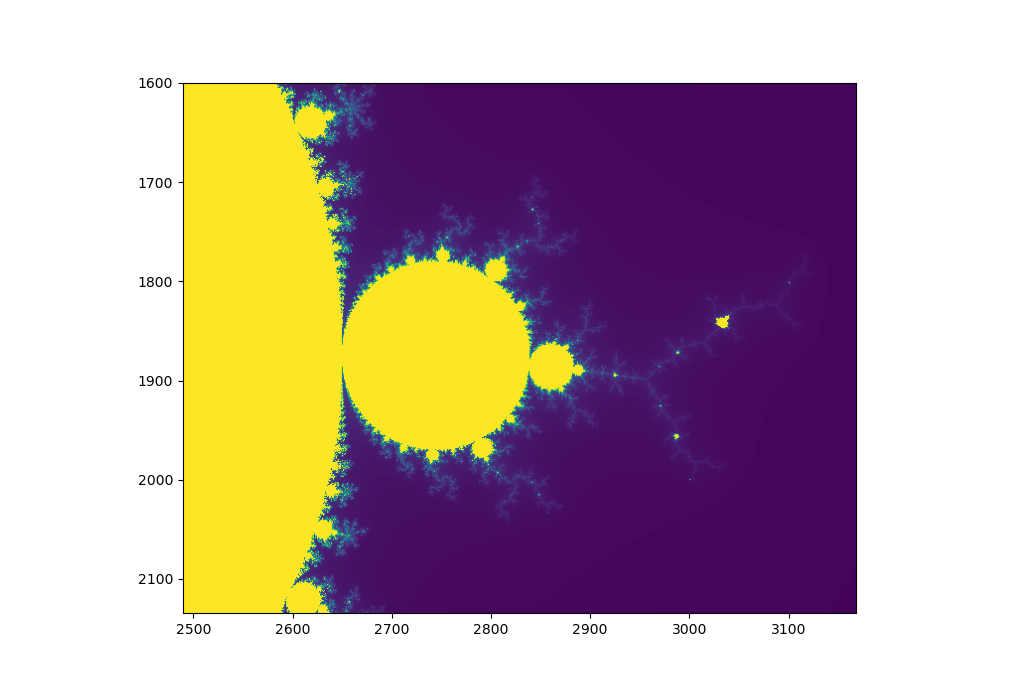
\includegraphics[width=0.7\textwidth]{mandelbrot_andrea.png}\hfill%




\end{enumerate}

\subsection*{Andere Aufgaben}

\begin{enumerate}[1.]
\setcounter{enumi}{6}

\item \textbf{ggT}\\
Schreiben Sie eine Funktion, die den größten gemeinsamen Teiler (ggT)
zweier Zahlen rekursiv berechnet. Schlagen Sie dazu, wenn nötig, den
``euklidischen Algorithmus`` nach.
\item \textbf{Minimum suchen}\\
Schreiben Sie eine Funktion \texttt{finde\_minimum(f,x0,x1,feinheit=$0.01$)}. Dabei ist $f$ eine Funktion (die ein reelles 
Argument hat und eine reelle Zahl liefert), x0 und x1 sind die Ränder des Intervals, in dem wie ein
Minimum suchen, \texttt{feinheit} die Feinheit der Unterteilung des Intervalls, die wir bei der Suche verwenden.
(Eine Aussage über die Genauigkeit des so gefundenen Minimums können Sie nur treffen, wenn Sie 
noch mehr über die Funktion wissen. Können Sie einen Satz formulieren und beweisen, der Bedingungen
formuliert dafür, dass ein so gefundene Minimalstelle einen Fehler von höchstens $\epsilon$ hat?)
Testen Sie ihre Funktion an der Kosinus-Funktion im Intervall $[2,4]$. 


%\item \textbf{Polygone}\\
%Lösen Sie die Aufgabe im Abschnitt 8.4 'Weiteres über Funktionen.'


%% \item \textbf{Anagramme}

%% Ein Anagramm ist ein Wort oder Satz, der durch Umstellen aller Buchstaben eines
%% anderen Satzes gebildet werden kann. Leerzeichen sowie Unterschiede zwischen Gro"s- und Kleinschreibung werden ignoriert. Beispiele sind die Paare \emph{Buecher sind Fre%unde} und \emph{Befreie den Urschund} oder \emph{Chaos} und \emph{Ach so}. Schreiben Sie ein Programm, das pr"uft ob zwei eingegebene Zeichenkette ein Anagramm von einander bilden. 

\item \textbf{Zeichnen} \\
Schreiben Sie ein Programm, das mit Turtle-Graphik zeichnet. Wenn Sie mit der Maus
an eine Stelle gehen und kicken, soll sich die Turtle zur neuen Position begeben und 
dabei zeichnen. Verwenden Sie dazu 
\begin{verbatim}
screen=turtle.Screen()
screen.onclick(...)
turtle.mainloop()
\end{verbatim}

Lesen Sie die Verwendung von 'onclick' in der Dokumentation nach.
Sie können sich
auch noch alle möglichen Erweiterungen ausdenken.


%% \item \textbf{Brown'sche Bewegung} \\ 
%% Schreiben Sie eine Funktion, die den Weg eines Teilchens in Brown'scher
%% Bewegung simuliert: Nehmen Sie an, dass das Teilchen  nach jedem Zeitschritt
%% in eine zufällige Richtung geht mit einer Schrittweite, die normalverteilt ist.
%% (In \texttt{numpy.random} gibt es die Funktion \texttt{normal}, die einen Wert
%% aus der Standard-Normalverteilung ausgibt.)  Die Funktion soll als Argument
%% die Anzahl der Zeitschritte akzeptieren und die Liste der vom Teilchen
%% betretenen Punkte zurückgeben. Der Pfad des Teilchens soll mit Hilfe
%% der Turtle-Graphik angezeigt werden. \\
%% Möglicher Zusatz: Führen Sie eine gewisse Zahl von Simulationen mit demselben Startpunkt durch, berechnen
%% sie den Mittelwert des Quadrats des Abstands zum Ausgangspunkt in Abhängigkeit von der Zeit $t$.
%% Veraunschaulichen Sie diese Abhängigkeit durch einen Plot.  Einsteins theoretische Voraussage
%% dieses Zusammenhangs war eine der drei Arbeiten, die ihm den Nobelpreis eintrugen.


\item \textbf{Kochkurve} \\
Die Kochkurve ist eine fraktale Kurve, die 1904 vom Schwedischen
Mathematiker Helge von Koch eingef"uhrt wurde. Bei jedem
Rekursionsschritt wird jede Strecke in drei Teile geteilt und die
mittlere Teilstrecke durch zwei Strecken ersetzt, die im Winkel von
$60^{\circ}$ anliegen.

\begin{center}
  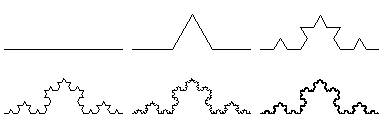
\includegraphics[width=0.5\textwidth]{gfx/koch-recursion}\hfill%
  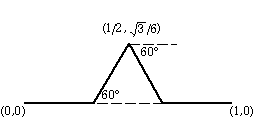
\includegraphics[width=0.4\textwidth]{gfx/koch-dent}\\
  {Links: Rekursionstiefen 0 bis 5 der Kochkurve. Rechts: Rekursionsschritt}
\end{center}

Schreiben Sie ein Programm, das eine Rekursionstiefe n einliest (und
eventuell noch eine Streckenl"ange f"ur den letzten Rekursionsschritt)
und die sich ergebende Kochkurve mit der Turtlegrafik malt.


\begin{center}
  
\includegraphics[width=0.2\textwidth]{gfx/koch-snowflake}\\
  {\glqq Schneeflockenkurve\grqq: Aus Kochkurven kann man eine
    Schneeflocke zusammensetzen}
\end{center}

% \item \textbf{Messwerte zeichnen} (zählt doppelt)\\

% Schreiben Sie eine Funktion \texttt{set\_point}, die als Argument  zwei Zahlen
% $x,y$ nimmt und  ein kleines Kreuz an der Stelle $x,y$ malt. (Die Koordinaten beziehen
% sich auf ein durch \texttt{turtle.setworldcoordinates} bestimmbares Koordinatensystem,
% schlagen Sie diese Funktion nach.) Als optionalen (key word-) Parameter soll die Funktionen
% die Länge der Balken des Kreuzchens enthalten.

% Schreiben Sie anschließend eine Funktion \texttt{draw\_axes}, die als Argument zwei Zahlen $a,b$ akzeptiert
% und anschließend Koordinatenachsen zeichnet mit Markierungen im Abstand $a$ (für die x-Achse)
% bzw. $b$ (für die y-Achse). Sie können die Markierungen mit Hilfe von
% \texttt{turtle.write(...)} beschriften. (Dies ist wieder bezogen auf das gegenwärtige Koordinatensystem).

% Schreiben Sie als drittes eine Funktion \texttt{draw\_data(l)}, die eine Liste
% von Wertepaaren einliest, das Koordinatensystem so einstellt, das alle Punkte
% darin Platz haben, anschließend die Achsen mir sinnvollen Markierungen zeichnet
% und die Punkte einzeichnet.

% Schreiben Sie als viertes eine Funktion \texttt{plot\_function(f,x0,x1)}, die ein
% Funktion $f$ im Intervall $[x0,x1]$ zeichnet.  Verwenden Sie dazu die vorige Funktion.

% Verwenden Sie für alle Funktionen Turtle-Graphik. 
% Testen Sie beim Programmieren jede der Funktionen separat!

\item \textbf{Damenproblem $^*$} (zählt doppelt)\\
Beim 8-Damenproblem geht es darum, 8 Damen auf einem Schachbrett ($8*8$
Felder) so zu setzen, dass keine Dame von einer anderen geschlagen
werden kann (d.\,h. keine zwei Damen sind in einer Zeile, Spalte oder
Diagonalen). Allgemeiner formuliert setzt man beim
$n$-Damenproblem $n$ Damen auf einem Brett mit $n$*$n$ Feldern.

Das Problem kann man mit \emph{Backtracking} l"osen. Dabei setzt man
rekursiv eine Dame nach der anderen. Wenn eine neu gesetzte Dame
eine der bereits gesetzten Damen schlagen k"onnte, so wird der Zug
zur"uckgenommen und die n"achste m"ogliche Position f"ur die Dame wird
ausprobiert. Ebenso wird, wenn es f"ur die rekursiv nachfolgenden
Damen keine L"osung gibt, die Dame zur"uckgenommen und die folgende
Position versucht. Aufgrund des Zur"ucksetzens wird der Ansatz als
Backtracking bezeichnet.

Man beachte hier, dass man f"ur jede Zeile (oder Spalte) von vorne
herein nur eine Dame platzieren muss.




% \item \textbf{1D-Zellularautomaten mit ASCII-Graphik} (zählt doppelt)

% Stellen Sie Sich eine Reihe von Zellen vor, die in einer Linie
% nebeneinander liegen.  Jede Zelle hat einen Zustand, tot oder
% lebendig.  Nun sollen sich die Zust"ande der Zellen in der Zeit
% schrittweise ver"andern, und zwar ist der Zustand abh"angig von dem
% alten Zustand und den Zustand der beiden benachbarten Zellen.

% Den \emph{Zustand} von je drei Zellen kann man als eine Zahl von 0 bis 7 
% auffassen: die Zust"ande als 0/1-Ziffern der Bin"arcodierung. Zum Beispiel
% Tot-Lebendig-Tod entspricht $010_2 = 2$.
% %
% Eine \emph{Regel} f"ur den zellul"aren Automaten definiert nun f"ur jeden 
% Zellenzustand  unter Ber"ucksichtigung ihrer Nachbarn, d.h. es ergibt sich
% eine Tabelle mit acht Eintr"agen.
% %\vspace{1ex} \noindent

% \begin{minipage}{\textwidth}
%   Bsp.: 
%   \begin{minipage}{0.45\textwidth}
%     \begin{center}
% \begin{tabular}{r@{ = }l|c}
% \multicolumn{2}{c|}{Nachbarschaft}&Nachfolger\\
% \hline
% LLL ($111_2$&$7$)& L (1) \\ 
% LLT ($110_2$&$6$)& T (0) \\ 
% LTL ($101_2$&$5$)& T (0) \\ 
% LTT ($100_2$&$4$)& L (1) \\ 
% TLL ($111_2$&$3$)& T (0) \\ 
% TLT ($010_2$&$2$)& L (1) \\ 
% TTL ($001_2$&$1$)& L (1) \\ 
% TTT ($000_2$&$0$)& T (0) \\ 
% \end{tabular}
%     \end{center}
%   \end{minipage}
% \hfill
%   \begin{minipage}{0.45\textwidth}
%     \begin{center}
%        %\input{gfx/ueb/1d-cells-rule.latex}
%        \includegraphics[width=0.5\textwidth]{gfx/ueb/1d-cells-rule-notex}
%      \end{center}
%   \end{minipage}
% \end{minipage}

% \vspace{1ex} \noindent
% Damit kann man dann die Regel einfach als Folge von acht Bits auffassen,
% also als Zahl von 0 bis 255 (im Beispiel $10010110_2 = 150$).

% Schreiben Sie ein Programm, das eine Regel als Zahl 0 bis 255 
% einliest und die Entwicklung der Zellen in der Zeit berechnet. Geben Sie
% f"ur jeden Zeitschritt ({\em Generation}) die Zellen in einer Zeile aus,
% jede Zelle je nach Zustand als anderen Buchstaben.
% F"ur die Zellen am Rand ist es am einfachsten, wenn Sie die linkeste und 
% rechteste Zelle als benachbart ansehen (ein sog. \glqq wraparound\grqq).

% Die Anfangspopulation kann zuf"allig zuf"allig belegt werden. 


% \begin{center}
% \hfill
% \begin{minipage}{0.3\textwidth}
%   \begin{center}
%     \includegraphics[width=\textwidth]{gfx/ueb/shellcells}
% %  {\tiny Bildquelle:~\href{http://www.stephenwolfram.com/publications/articles/ca/83-cellular/2/text.html}{\url{stephenwolfram.com}}
%   {\tiny Bildquelle:~\href{http://www.stephenwolfram.com/publications/articles/ca/83-cellular/2/text.html}{StephenWolfram}}
%   \end{center}
% \end{minipage}
% \hfill
% \begin{minipage}{0.3\textwidth}
%   \begin{center}
%     \includegraphics[width=\textwidth]{gfx/ueb/cell122}
%   {\tiny Beispielausgabe f"ur Regel 122.
% }
%   \end{center}
% \end{minipage}
% \hfill
% \begin{minipage}{0.3\textwidth}
%   \begin{center}
%     %\includegraphics[width=\textwidth]{gfx/ueb/shellcells-flickr}
%     %{\tiny Bildquelle:~\href{http://flickr.com/photos/53447683@N00/68806485}{Flickr}}
%     \includegraphics[width=\textwidth]{gfx/ueb/SchneckeOlivia-Porphyria-MaxPlanckViaSpon.jpg}
%     {\tiny Bildquelle:~\href{http://www.spiegel.de/fotostrecke/fotostrecke-46503.html}{Max-Planck-Institut}} % f"ur Entwicklungsbiologie}}
%   \end{center}
% \end{minipage}
% \hfill
%   \end{center}

% F"ur einige Regeln "ahnlich die Ergebnisse Mustern auf manchen Muscheln.


\end{enumerate}
\subsection*{Aufgaben zu Numpy, Scipy, Matplotlib}
\begin{enumerate}[1.]
\setcounter{enumi}{10}

\item \textbf{Winkel berechnen}\\
Sehen Sie sich die Dokumentation des Pakets \texttt{numpy.linalg} an.
Schreiben Sie eine Funktion, die zwei Vektoren im $\R^n$ als Argumente
akzeptiert und den von den beiden Vektoren eingeschlossenen Winkel zurückgibt.

\item \textbf{Gleichungssystem  lösen, I}\\
Bestimmen Sie die Matrix der linearen Abbildung $\R^3\to \R^3$, die
die Punkte $\tvector{1\\2\\3},\tvector{1\\1\\0},\tvector{0\\0\\-1}$ auf die
Punkte $\tvector{2\\1\\1},\tvector{1\\0\\0},\tvector{0\\-1\\-1}$ abbildet.

\item \textbf{Gleichungssystem lösen, II}\\
Erstellen Sie für $n=2,3,4,10$ die Matrix $M=(m_{ij})_{1\leq i,j\leq n}$, $m_{i,j}=1/(i+j-1)$. (Beachten
Sie, dass numpy-Arrays die Indizierung bei Null beginnen lassen, während man 
in der Mathematik mit 1 anfängt.)  Lösen Sie das Gleichungssystem $Mx=\tvector{1\\1\\ \ldots \\1}$.
Machen Sie jeweils die Probe, um festzustellen, ob die Lösung tatsächlich eine ist. Was fällt
Ihnen auf für $n=10$? 

\item \textbf{Schwerpunkt, Trägheitstensor $^*$} (zählt doppelt)\\
Schreiben Sie eine Funktion, die eine Liste von Vektoren im $\R^3$ akzeptiert
und daraus den Schwerpunkt und  den Trägheitstensor, sowie
die Eigenvektoren des Trägheitstensors berechnet. Zusatz$^*$:  Visualisieren Sie das.

\item \textbf{Mittelwert und Varianz}\\
Schreiben Sie eine Funktion, der eine Liste von Zahlen übergeben wird, 
und die daraus Mittelwert und Standardabweichung berechnet.

\item \textbf{$\pi$ durch Zufallsexperiment $^*$} (zählt doppelt)\\
Ziehen Sie $N$ ($N=1000,10000,100000$) Punkte $(x_i,y_i)$ aus
dem Quadrat $[-1,1]\times[-1,1]$ (d.h. beide Koordinaten werden
aus einer Gleichverteilung über das Intervall $[-1,1]$ gezogen, 
siehe \texttt{numpy.random}). Zeigen Sie die gezogenen Punkte
in einer Graphik, wobei die Punkte innerhalb des Einheitskreises
eine andere Farbe haben sollen. Ermittelns Sie die Anzahl der Punkte $N_E$,
die innerhalb des Einheitskreises liegen und geben Sie 
$4\frac{N_E}{N}$ aus. (Welchen Wert erwarten Sie? Sie können auch versuchen,
sich zu überlegen, wie wahrscheinlich eine Abweichung von mehr als 1 Prozent
von dem erwarteten Wert ist.)

\item \textbf{Mikrozensus, I}\\
Verwenden Sie die Mikrozensusdaten in der Datei \texttt{algebuei.csv}
und lesen Sie sie mit Hilfe von \verb|numpy.genfromtxt| in ein
Array. Erstellen Sie ein Histogramm aller Einkommen, der 
Einkommen der Männer, der Einkommen der Frauen. Versuchen
Sie, beide Histogramme in einer Graphik mit 'gestapelten Balken'
anzuzeigen.

\item \textbf{Mikrozensus, II}\\
Bestimmen Sie den Mittelwert und den Median
des Einkommens für jedes Bundesland.
Stellen Sie die Ergebnisse in einer 
Graphik dar.

\item \textbf{Iris-Daten $^*$} (zählt doppelt)\\
Lesen Sie die Daten in \texttt{iris.csv} in ein
Array.  Sie stellen gemessene Längen und  Breiten von
Blütenblättern drei verschiedener Schwertlilienarten dar.
Stellen Sie die Daten als 3d-Punktwolke bezüglich drei
der vier Parameter dar, wobei die Farbe der Punkte die
Art bezeichnen soll.  
\end{enumerate}
\end{document}
